\section{Introduction}

\textbf{Goal of course:} Understand principles of user-centered design and able to apply these to practice.
Learn about the basic notions of Computational Design in HCI context. \medskip


\textbf{Moore's Law}
Computational power grow exponentionally. Transistor count doubles every two years. Also with RAM and pixel densities. 
However: Human capabilities stay stable.\medskip

\textbf{Good System design}
Accounts for human capabilities, human error and exceptional circumstances. \medskip

\textbf{Human Computer Interaction}
Concerned with design, evaluation and implementation of interactive computing systems for human use. \medskip

\textbf{Process in HCI}

\begin{center}
	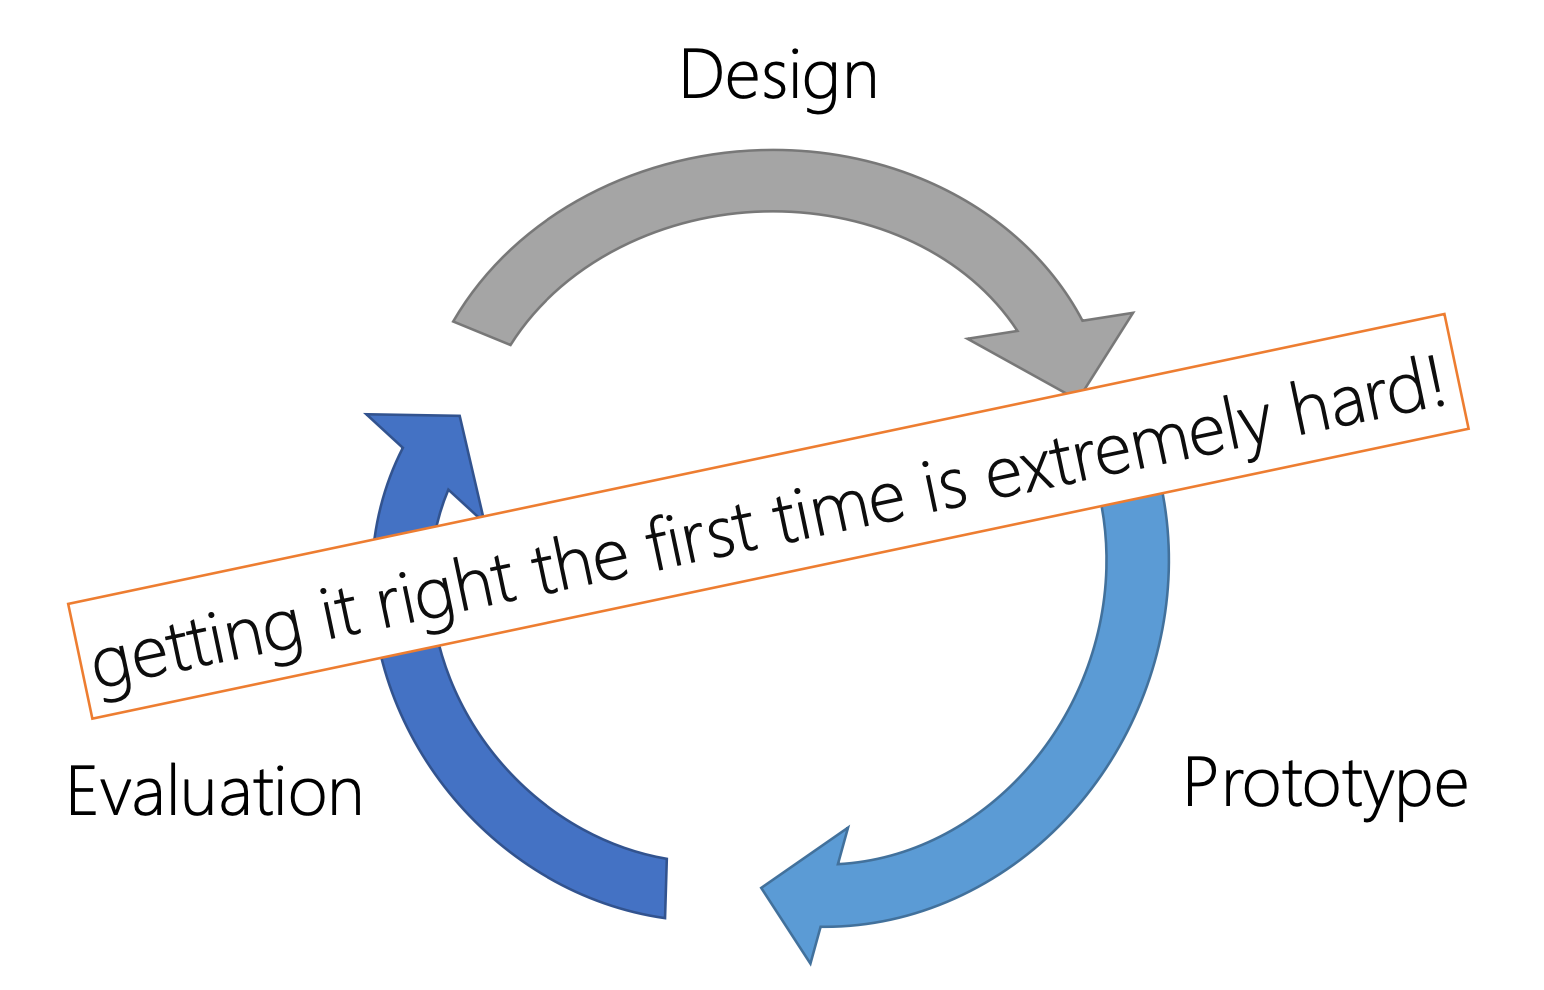
\includegraphics[width=\linewidth]{process.png}
\end{center}

Formative : understand problem and user to inform our design. \medskip
Evaluative: understand how well design works. Also detects mistakes in design. \medskip

